\section{Sentiment analysis recensioni}\label{SentimentAnalysis}
La sentiment analysis sulle recensioni è stata affrontata sotto diversi aspetti per raggiungere tre obiettivi principali. Il primo obiettivo è stato quello di verificare la corrispondenza tra la positività individuata dal numero di stelle e la polarità ottenuta tramite un approccio basato sul lessico. Il secondo obiettivo è stato quello di capire quale fosse il sentimento medio delle 3 stelle, le quali dovrebbero corrispondere ad un voto neutro. Questo obiettivo nasce dal fatto che una recensione a 3 stelle, seppur neutra, possa presentare delle sfumature più tendenti al positivo o negativo (es: "Prodotto di qualità mediocre, ma per il prezzo che ha fa il suo lavoro... Consigliato per chi vuole spendere poco" e "Non è il massimo... ci sono alternative migliori sul mercato e non credo che lo ricomprerei." potrebbero essere recensioni da 3 stelle che esprimono sentimento diverso). Infine, come ultimo obiettivo è stato reputato interessente lo studio dell'evoluzione nel tempo del sentimento, rapportato anche all'evoluzione del numero di stelle, di alcuni prodotti d'esempio. 
\\\\
Nel seguito viene presentato il lavoro attraverso due approcci in quanto il primo (\ref{ApproccioLexiconBased}), basato sul lessico, ha portato a scarsi risultati, per cui ad esso è stato preferito un approccio basato sul machine learning (\ref{ApproccioMachineLearning}).
In entrambi gli approcci l'attributo della recensione su cui viene condotta l'analisi è quello del \textit{body}. È stato inoltre deciso di etichettare come positive le recensioni con \textit{rating} > 3 e come negative quelle con \textit{rating} < 3 per poter dare una stima dell'accuratezza dei risultati ottenuti.


\subsection{Approccio Lexicon Based}\ref{ApproccioLexiconBased}
La lingua italiana del dataset porta ad avere una cerchia più ristretta di alternative per effettuare una sentiment analysis. L'approccio che è stato adottato fa affidamento al lessico di Sentix, grazie al quale è stato possibile assegnare alle recensioni una polarità ottenuta dalla somma delle polarità delle parole considerate. Ogni record del lessico è costituito da un lemma, dal tipo (nome, verbo, aggettivo, ecc.) e da diversi scores\footnote{\url{http://valeriobasile.github.io/twita/sentix.html}}. 
\\\\
Questo metodo è stato testato su un campione casuale di 1000 recensioni etichettate come positive e 1000 come negative. Le recensioni in questione sono state estratte da un sottoinsieme attendibile, ottenuto tramite l'intersezione di quelle di acquisti verificati (\textit{verified = true}) e di quelle considerate utili da almeno un utente (\textit{helpful > 0}). Considerando come positive le recensioni con polarità > 0, come negative quelle con polarità < 0 e scartando quelle per cui Sentix non ha riscontrato parole nel lessico, si ottiene un'accuratezza pari a 0.605 . In tabella \ref{tab:matriceConfusione} è disponibile la matrice di confusione, dalla quale si può che la maggior parte delle recensioni venga classificata come positiva.

\begin{table}[]
    \centering
    \begin{tabular}{l|l|l|}
    \cline{2-3}
     & \textbf{NEG} & \textbf{POS} \\ \hline
    \multicolumn{1}{|l|}{\textbf{NEG}} & 279 & 718 \\ \hline
    \multicolumn{1}{|l|}{\textbf{POS}} & 68 & 929 \\ \hline
    \end{tabular}
    \caption{Matrice di confusione classificazione recensioni con Sentix}
    \label{tab:matriceConfusione}
\end{table}

È stato inoltre verificato che non ci fosse una correlazione tra i valori della polarità rispetto al rating, sia aggregato per 1-2 e 4-5 stelle che preso singolarmente. Questo per stabilire se le polarità potessero essere coerenti con il rating considerando un intervallo di valori diverso per distinguere recensioni positive e negative. I valori ottenuti come coefficiente di correlazione di Pearson sono rispettivamente di 0.369 e 0.347, quindi si può concludere che non ci sia correlazione.
\\\\
Gli scarsi risultati hanno portato a scartare l'approccio e a prenderne in considerazione uno alternativo per poter perseguire gli obiettivi preposti sulla tendenza di utilizzo delle 3 stelle e sull'andamento della polarità nel tempo.

\subsection{Approccio Machine Learning}\label{ApproccioMachineLearning}
%TODO: dire che si considera il binario, GABRI the machine learner se ha in mente premesse da fare le facci lei
%TODO: dire modello utilizzato e con che parametri eventualmente

Anche in questo caso, avendo a disposizione un numero di recensioni molto elevato, si è deciso di utilizzare il sottoinsieme filtrato su quelle che sono sia verificate che considerate utili da almeno un utente in quanto considerate più affidabili per addestrare il modello. Per bilanciare il numero di recensioni positive molto più alto di quelle negative da dare in input al modello è stato fatto undersampling ed è stato ottenuto un insieme di XXX esempi di training diviso in due tra le classi. \\
Il modello è stato addestrato tramite una 10-fold cross-validation ed ha ottenuto un'accuratezza pari a XXX, con la matrice di confusione riportata in tabella \ref{tab:matriceConfusioneModello}. \\\\
%TODO: tab:matriceConfusioneModello
%AAAAAAAAAAAAAAAA: da qui in poi i risultati che mostriamo dovremmo tirarli fuori dalle recensioni non filtrate

Con il modello ottenuto è stato poi possibile calcolare il sentimento delle recensioni su alcuni prodotti d'esempio per osservarne l'andamento nel tempo rispetto al trend delle stelle. In questo caso, per avere un insieme di valori più ampio e tracciare un grafico migliore, sono state considerate anche le recensioni non verificate e non marcate come utili. Dopo aver effettuato la previsione del sentimento, è stata calcolata la media dei valori raggruppati per mese ed è stata tracciata la curva nel tempo. Come si può vedere in figura \ref{fig:andamentoSentimentoProdotto}, la curva del sentimento e quella del numero medio di stelle\footnote{i valori medi del numero di stelle sono stati portati in una scala compresa tra 0 e 1} seguono lo stesso andamento. Inoltre, è stato calcolato un valore per rappresentare il trend della curva del sentimento, il quale corrisponde al coefficiente angolare della retta che meglio approssima la curva. Dato un prodotto, è quindi possibile verificare se il sentimento delle recensioni sia in crescita o meno. \\\\

\begin{figure}[]
    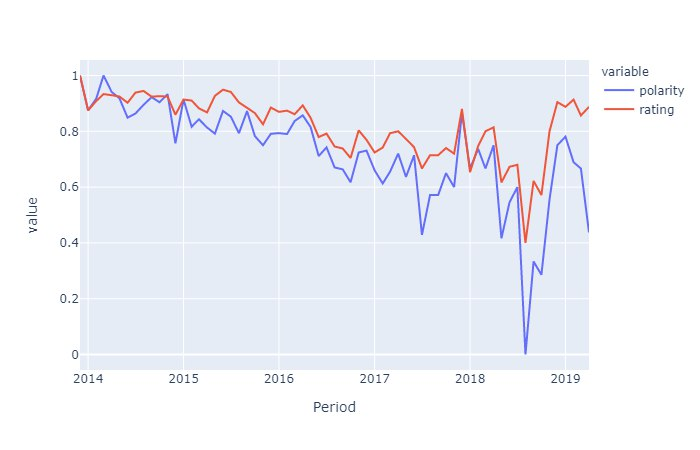
\includegraphics[scale=0.45]{andamentoSentimentoProdotto}\centering
    \caption{Andamento di sentimento e numero di stelle nel tempo per il prodotto "Kingston Dtig4/32Gb Datatraveler Memoria Flash, US"}\label{fig:andamentoSentimentoProdotto}
\end{figure}

Come ultima cosa, è stato utilizzato il modello per verifiare il sentimento medio rispetto all'utilizzo delle 3 stelle. I risultati ottenuti mostrano come il 46.8\% delle recensioni sia positivo, dimostrando quindi che non ci sia una tendenza dominante verso un sentimento.


